The relevant points for the given functions are as follows:\\
Graph 1:\\
$f(x)$ has local maxima and minima in $x=(-1)$ and $x=1$.\\
$f(x)$ decreases when approaching $f(-1)$, increases between $f(-1)$ and $f(1)$, and again decreases following $f(1)$.\\
Graph 2:\\
$f(x)$ has local maxima in $f(a)$, where $a \in [-1,0]$ and $f(b)$, where $b \in [0,3]$.\\
$f(x)$ has a local minimum in $f(0)$\\
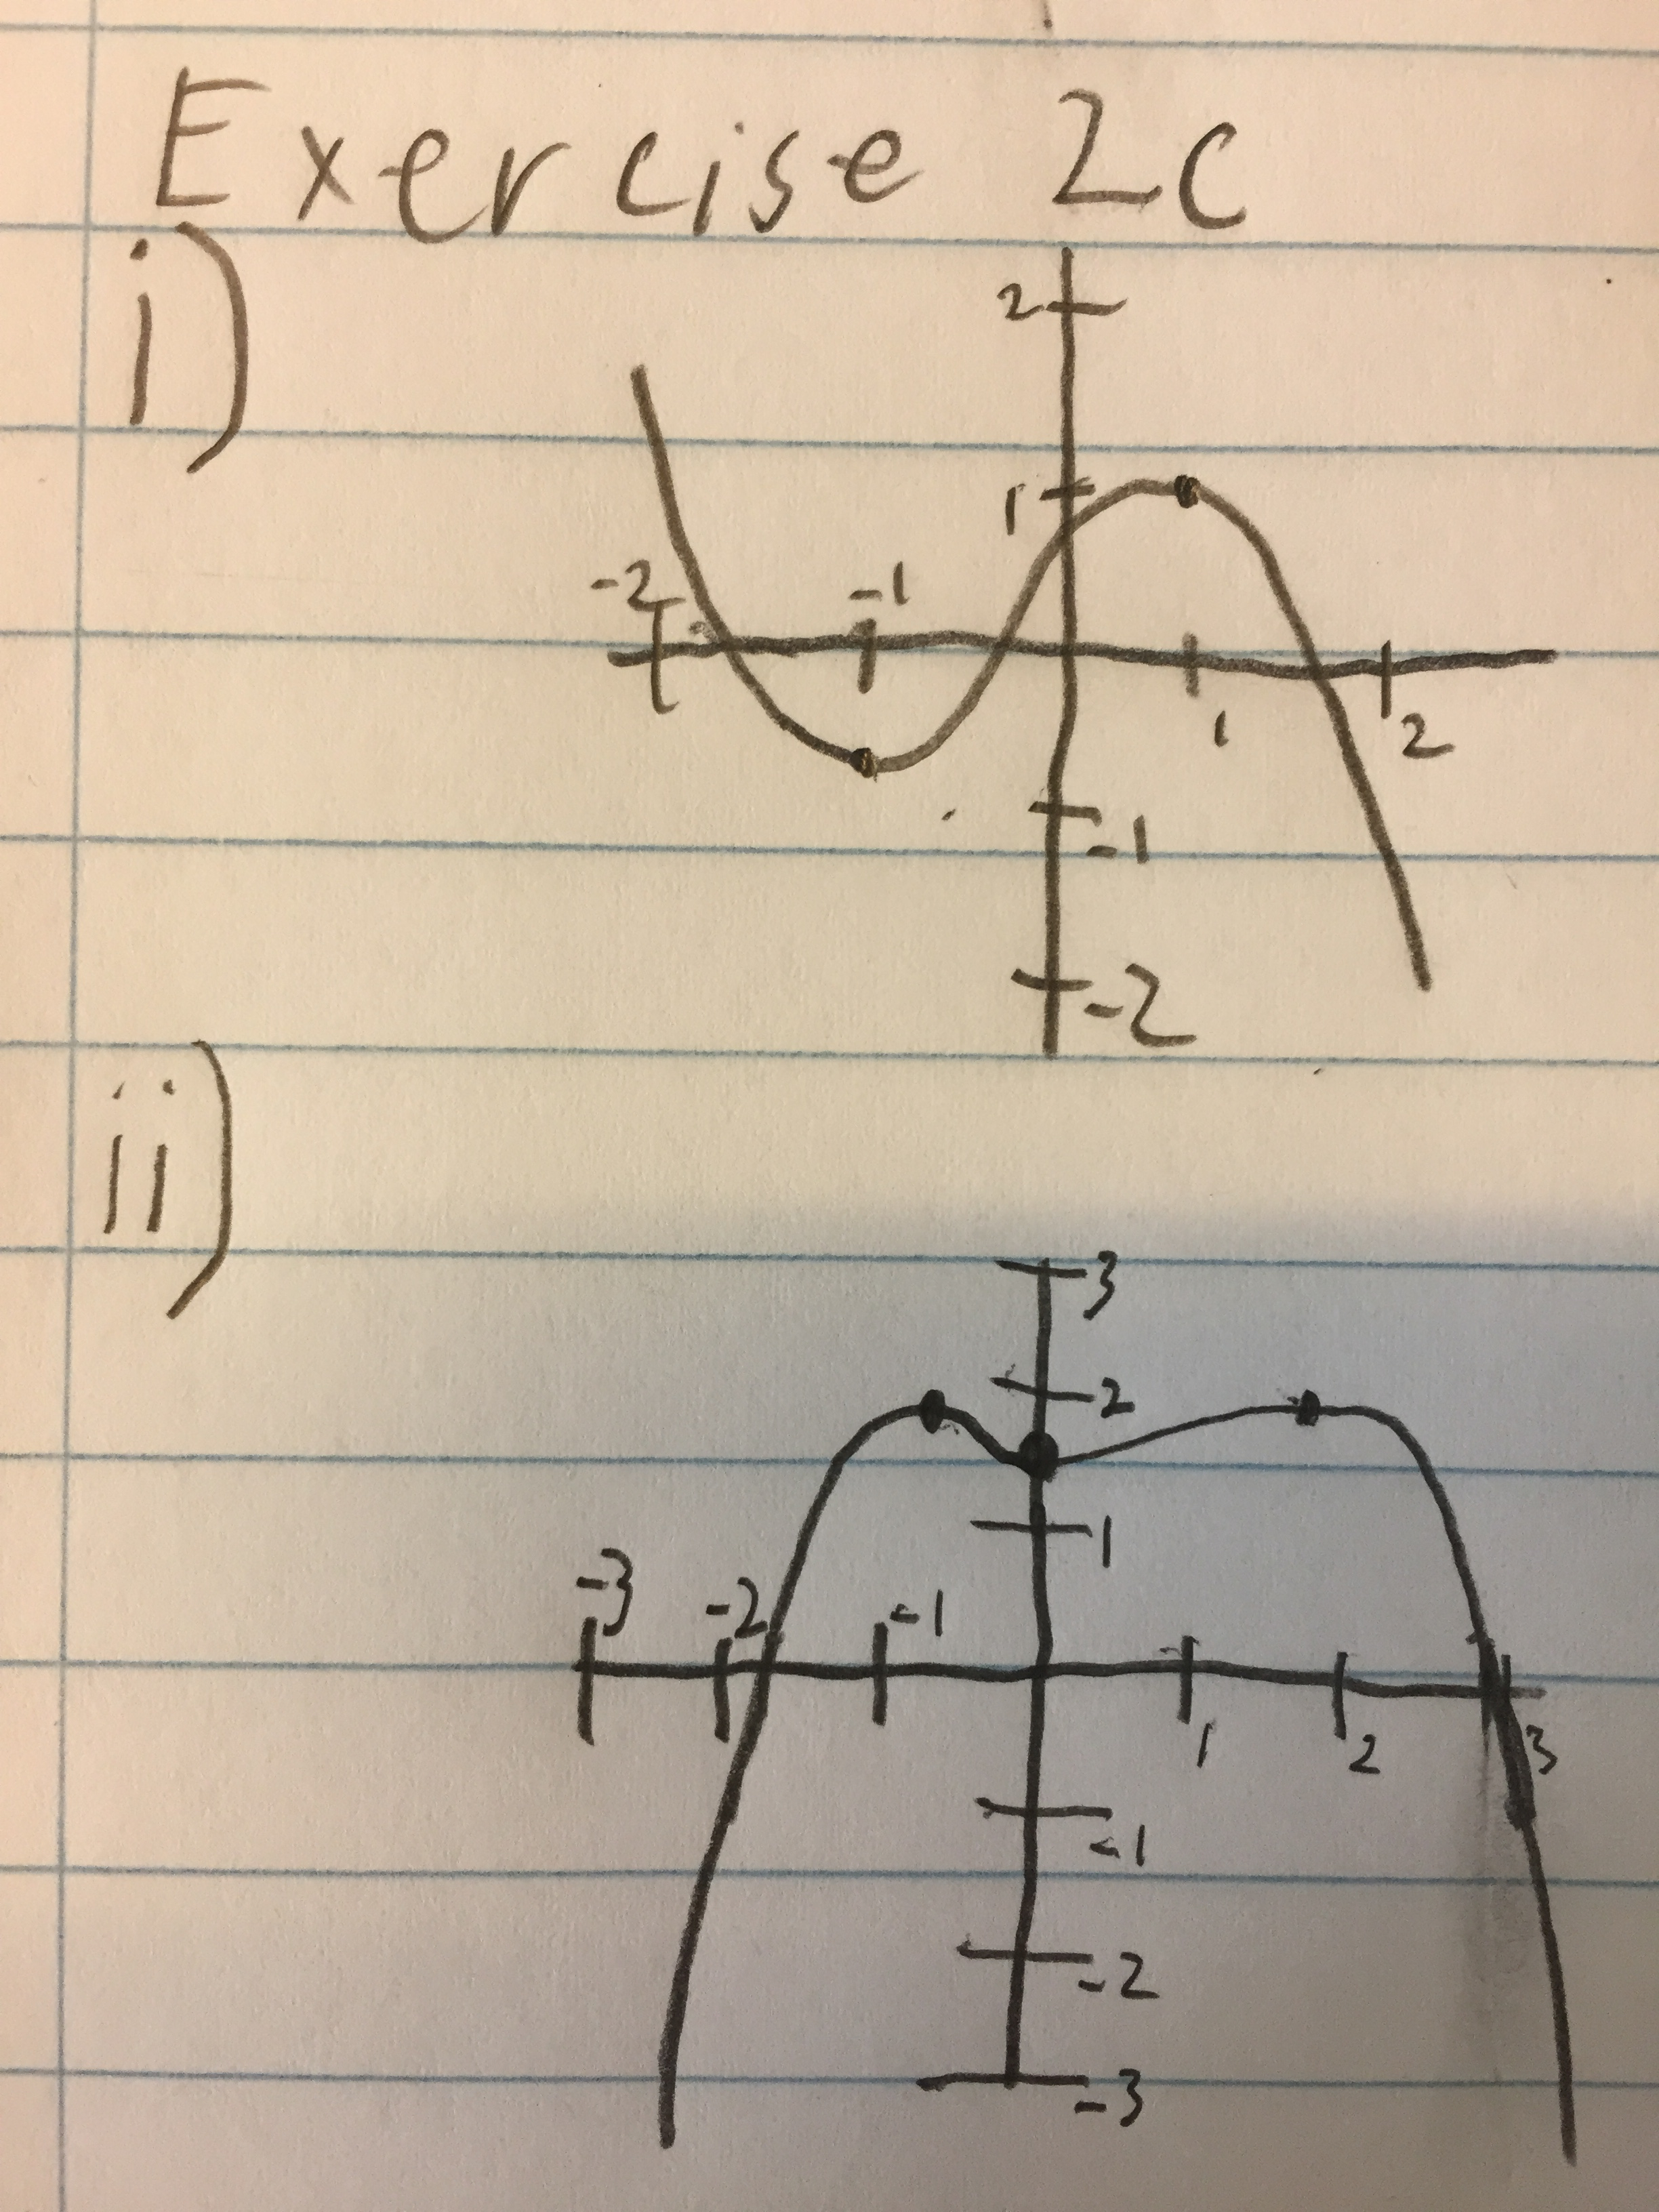
\includegraphics[width=0.5\linewidth]{masd2c.jpg}